\documentclass[twocolumn]{report}
\usepackage{graphicx}
\usepackage{tocloft}
\usepackage{placeins}
\usepackage{siunitx}
\graphicspath{ {./images/} }

\title{\textbf{Dynamic Audio System Based On Listener's Position For Surround Sound Effect}}
\author{Nachiket Kamod (12), N V Roshni (31),\\Ganeshsai Muppasani (30), Jagrati Chowdhari (9), \\\\\textbf{Guided By,}\\Prof. Deepali Yewale}
\date{\textbf{Academic Year}\\2020 - 21}

\begin{document}

\maketitle

\tableofcontents

\listoffigures

\chapter{}

\section{INTRODUCTION}

Automation plays an important role in the world 
economy and in daily experience in the last few 
decades has witnessed a rapid development in audio
systems.

Journey of audio systems begins with single channel 
audio system (monaural audio system) in year 1877, 
later in the year 1931 two channel Audio system 
(Stereo audio system) were introduced and in the year 
2005 the most advanced air audio or surround sound 
system (Multichannel audio system) were introduced.

Modern sound systems are increasingly gaining 
popularity day by day, particularly since technical 
advances have lowered their prices, increased their
qualities and features. One barrier to the greater 
experience while using these sound systems is its 
static nature in case of surround sound. Surround 
sound is a system of stereophony involving three or 
more speakers surrounding the listener so as to give a 
more realistic effect.

Even though high end audio systems provide good quality 
of sound but to achieve the surround sound effect the 
user has to configure the system manually depending 
upon his current position which is a very Tedious task.
Whenever you are settling up your complex home theatre 
bundle, understanding the art and science of speaker 
channel and placement is the most critical step in enjoying 
your new sound system.

Current sound system needs manual setup according to the 
ideal sitting position to achieve a good sound effect at 
fixed position. This manual setup consists of speaker angles 
and speaker sound adjusted to create and sound pocket around 
fixed position. But this effect varies when we move away
from the surround sound pocket created by speakers.

The aim of this project is to develop a real time system to 
determine the listener’s position and distance from the speaker 
system. The real time system described here is based on 
ultrasonic sensors mounted onto servo motors controlled by 
separate micro controllers (slave). The core of the system
is a master micro-controller termed as an audio processing 
unit which controls the speaker direction as well as sound levels. 
Distance measured from the rotating ultrasonic system, allows us 
to map 2 dimensional maps of the room in real time. With less 
system requirements, the surround sound pocket can be
adjusted according to the listener's position.

\section{ABSTRACT}

To explain the problem statement briefly, 
consider a real life scenario, I configured the 
orientation and volume levels of my sound system in 
order to get perfect surround sound at some 
position where I usually seat. But, now I want 
to change my seating position or even arrangement 
to some other part of my room which can be far 
right or left or may  be forward  or backward 
from the last seating arrangement. In this case 
to get perfect surround  sound I need to 
reconfigure my speakers again, that is, its 
orientation and volume levels as per the new 
seating position either with the help of technician 
or self which is mostly manual adjustments.

To overcome this scenario we experimented a combination of 
stereo vision and hardware technology which responds to real time
movements of listener and dynamically adjust the sound pocket. This system
uses opencv face detection algorithm and simple geometrical formula to
calculate depths and angles for individual speaker to introduce dynamically
adjusted surround sound. Since the system avoids the heavy usage of hardware, complex
algorithms and machine learning approach it can be implemnted on low powered
micorprocessors as well same processors used by sound systems.

\chapter{LITERATURE SURVEY}

\begin{description}
    \item[A.]\textbf{Surround sound systems}\\(United States Patents On, September 16, 2014)
\end{description}

This paper propses an idea of developing a system that comprises of 
reciever for receiving a multichannel spatial signal that comprises
at least one surround channel.

This system comprises of a directional  ultrasonic transducer for 
emitting ultrasound towards surface to reach a listening position via 
a reflection of the surface and a driver ckt to drive ultrasonic transducer.

The proposed system is capable of producing virtual surround sound without 
requiring a speaker a speaker to be located .

\begin{description}
    \item[B.]\textbf{Shadow Sound System Embodied with Directional Ultrasonic Speaker}\\(ICISA.2013 on 2013) 
\end{description}

The paper talks about usage of ultrasonic speaker and computer vision 
system installed on a motorized mount that can freely change the 
speaker’s directions and altitude for a specific registered user.

The resulting system is proven to be able to track the registered 
user for providing user selected sound contents without being 
interfered by other people.

This method seems promising but it requires individual hardware 
for each speaker and the solution does not cover the implementation 
on multi channel audio system efficiently.

\begin{description}
    \item[C.]\textbf{An Efficient Implementation of Acoustic Crosstalk Cancellation for 3D Audio Rendering}\\(IEEE China SIP on July 2014)    
\end{description}

In this paper given method the use of ultrasonic speaker and computer 
vision system installed on a motorized mount that can freely change 
the speaker’s directions and altitude for a specific registered user.

The resulting system is proven to be able to track the registered user 
for providing user selected sound contents without being interfered 
by other people.

This method seems promising but it requires individual hardware for 
each speaker and the solution does not cover the implementation on 
multi channel audio system efficiently.

\begin{description}
    \item[D.]\textbf{Multirate adaptive filtering for immersive audio}\\(IEEE Xplore  on February 2001)
\end{description}

This paper describes a method for implementing immersive audio 
rendering filters for single or multiple listeners and loudspeakers.

In particular, the paper is focused on the case of single or two 
listeners with different loudspeaker arrays to determine the weighting 
vectors for the necessary FIR and IIR filters using the LMS (least-mean-squares) 
adaptive inverse algorithm.

It describes transform-domain LMS adaptive inverse algorithm that is 
designed for crosstalk cancellation necessary in loudspeaker-based 
immersive audio rendering. 

The algorithm used in this paper is only for single listener and 
only two loudspeakers are used.

\section{CONCLUSION}

High end audio systems provide a very high-quality sound and provides 
the user the feasibility to use them for multiple events. But even the 
best has some drawbacks.

\begin{description}
    \item[-]Complexity of Hardware, as per the research study we can 
            observe the research is based on mono channel and not multi channel. 
    \item[-]Research suggests use of kinect for object tracking which have its 
            own drawbacks.
    \item[-]Complexity of Algorithm, to achieve the effect researchers suggested 
            very complex algorithms regardless of room geometry.
\end{description}

\chapter{AIM AND OBJECTIVES}

\section{Aim}

To develop a real time self adjusting Audio system based on listener's 
position to achieve high quality air sound effect.

\section{Objectives}

\begin{description}
    \item[1.]To introduce automation into current trend of audio system.
    \item[2.]To make the audio system compatible of adjusting it’s 
                orientation or direction and sound intensity based on user's 
                position.
\end{description}

\section{Methodology}

From abstract we can conclude speaker angles and sound intensities of individual 
speakers are very much important.

Speaker angles defines how the sound is gonna reach to the listener. Like is it 
reflecting from any surface or the sound source is directly pointed towards the listener.

Sound is nothing but oscillations of particles (typically air) in vibrational motion, which
transports energy through a medium.

\begin{figure}
    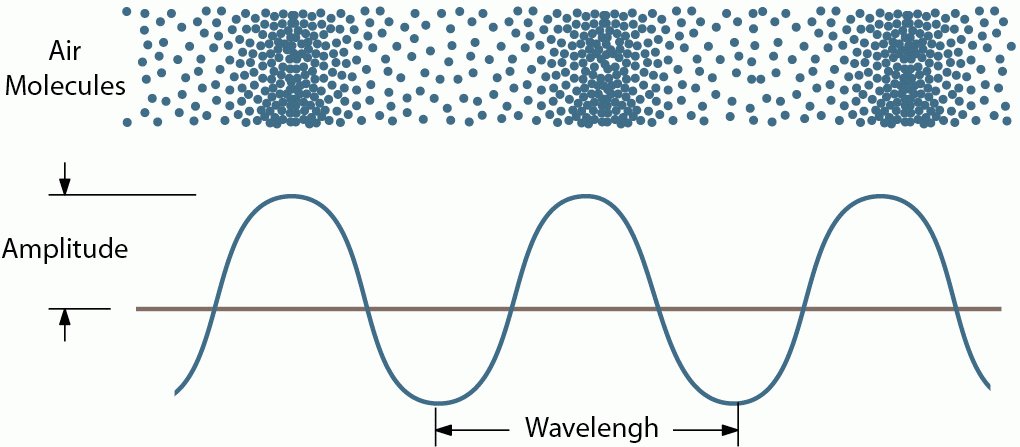
\includegraphics[width=\columnwidth]{sound_waves.png}
    \caption{Sound Waves}
\end{figure}

\FloatBarrier

Speakers push and pull surround air molecules in waves to generate a sound wave using a diaphragm.
Typically, this diaphragm is in conical shape hence it oscillates the molecules in the oval field. 

\begin{figure*}[ht]
    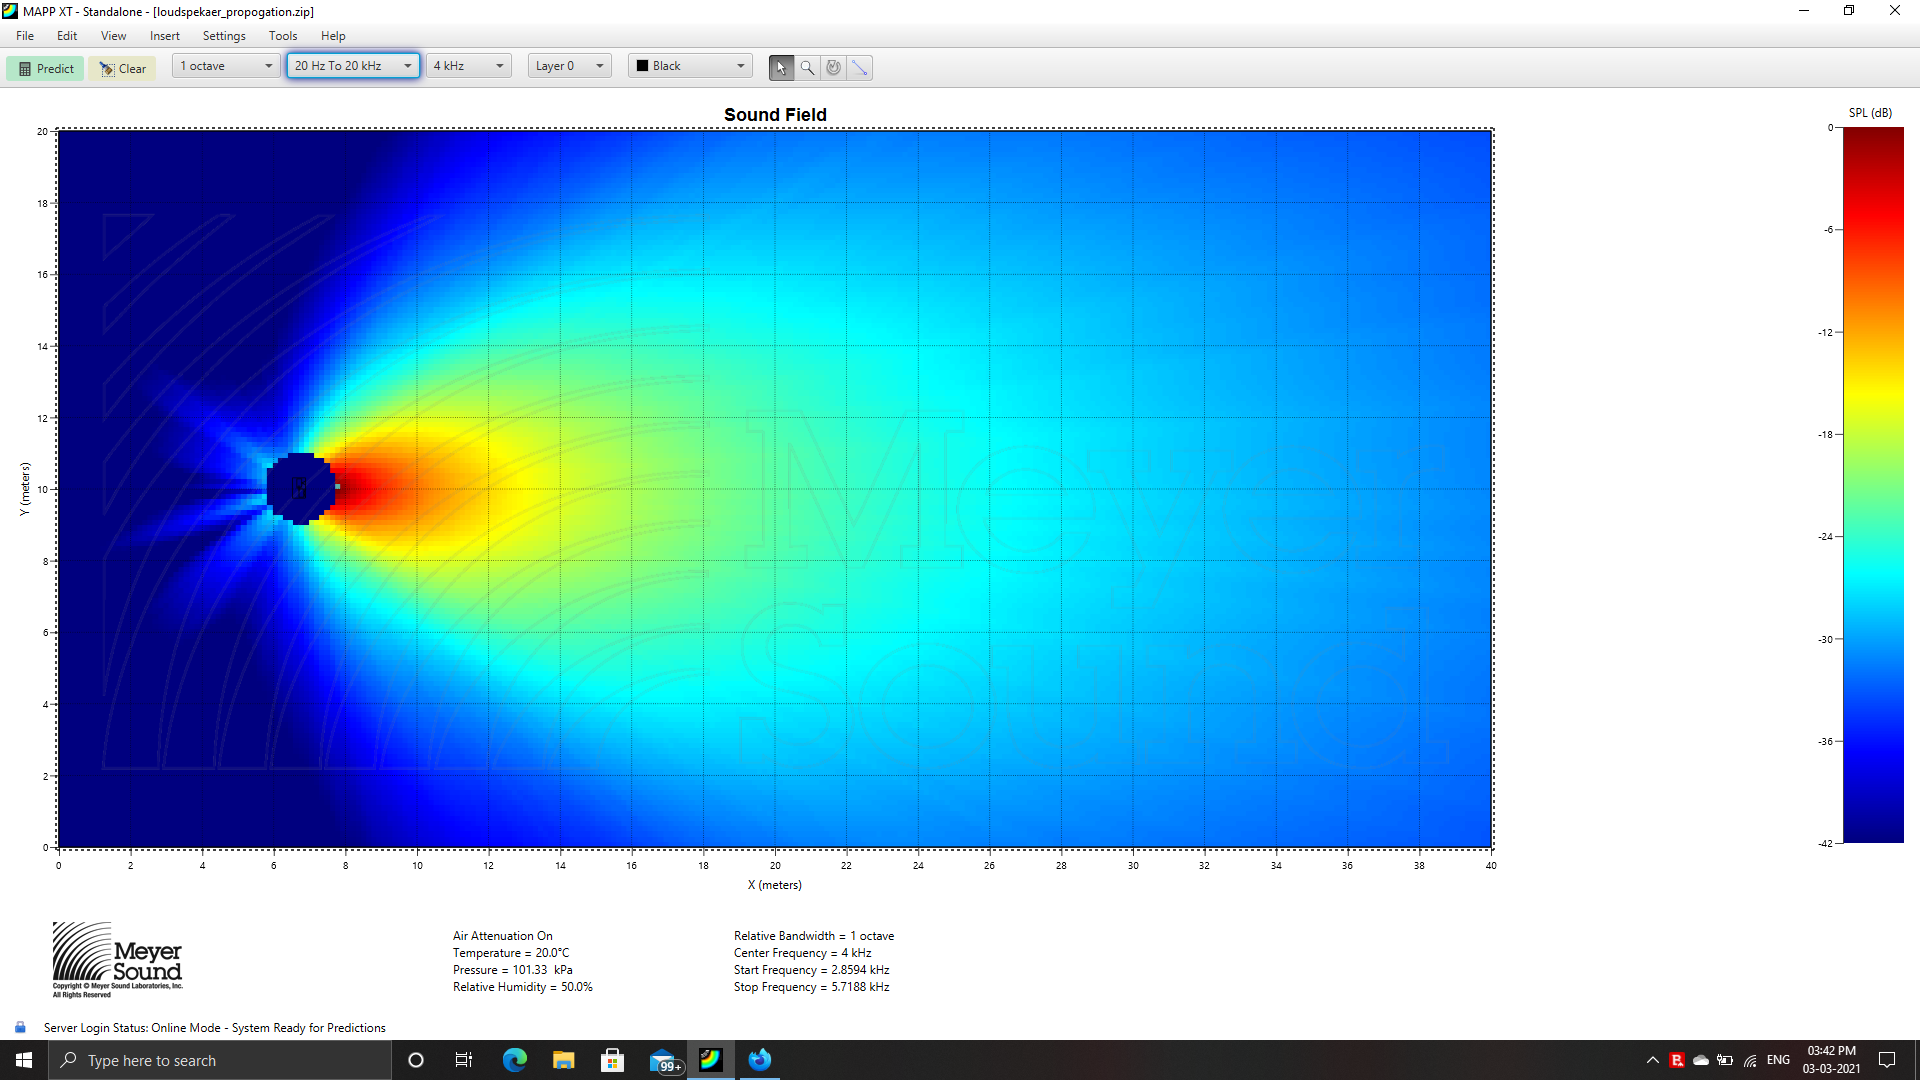
\includegraphics[width=1\textwidth]{sound_propogation_for_speaker.png}
    \caption{Sound propgation of speaker}
\end{figure*}

\FloatBarrier

Figure 3.2 shows the oval propgation of the sound field from the speaker. Where sound
intensity of speaker at some depth is denoted with heat map (dB). In front of the speaker
the sound intensity is maximum and it fades away as we go far away from the speaker. Where 
in the other hand it is much less at the back of the speaker. Since, it is oval in nature, 
the propogation to left and right is also less than that of front.

Figure 3.3 shows the reflection and reverberation of sound due to misalignment
and excessive sound intensity of speaker due to collision of sound waves onto walls. 
These reflections build up with each reflection and decay gradually as they are absorbed by the surfaces of Objects and walls
in the room. In this case, listener tends to hear direct sound and the repeated
reflected sound waves which might sound muddy and grabbled.

\begin{figure}
    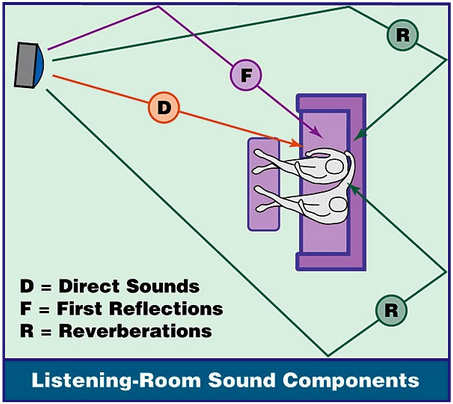
\includegraphics[width=\columnwidth]{reverberation.png}
    \caption{Reflection and reverberation of sound}
\end{figure}

\FloatBarrier

Hence, it becomes necessity to align the speakers as well as adjust the sound levels
in proper amounts to get best surround sound.

To overcome this scenario we experimented a five
block system. Which consists of,

\begin{description}
    \item[1.]Depth estimation unit (Cameras), to measure the depth of the listener
            from one reference point and feed these varibles to microporcessor for 
            further calculations.
    \item[2.]Microprocessor, to measure depth and calculate 
            panning and tilting angles as well as listener's depth
            from each speaker.
    \item[3.]Mechanical unit, to pan and tilt the speakers.
    \item[4.]Audio Processor Unit (Digitally controlled amplifier),
            to adjust the individual speaker gain using calculated 
            results from microporcessor.
    \item[5.]Speakers, to sound individual 4 channeled output.
\end{description} 

\section{Specifications of the System}

\subsection{Depth estimation unit}

Depth estimation unit includes stereo vision assembly of two web cams with similar 
(known or unknown) focal length (In our case 18 cm).

\begin{figure}[h]
    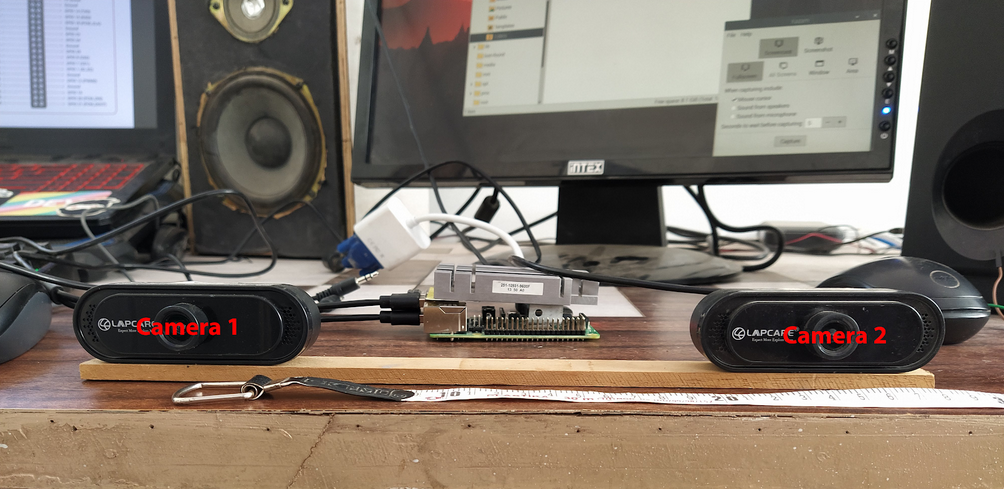
\includegraphics[width=\columnwidth]{assembly.png}
    \caption{Assembly of the depth estimation unit}
\end{figure}

Placed at some known distance \(x \) from each other (24 cm).

\subsection{Microprocessor}

Microprocessor serves an important role in DAC appplication, data processing estimation 
and controlling the response hardware in real time.

\begin{figure}[h]
    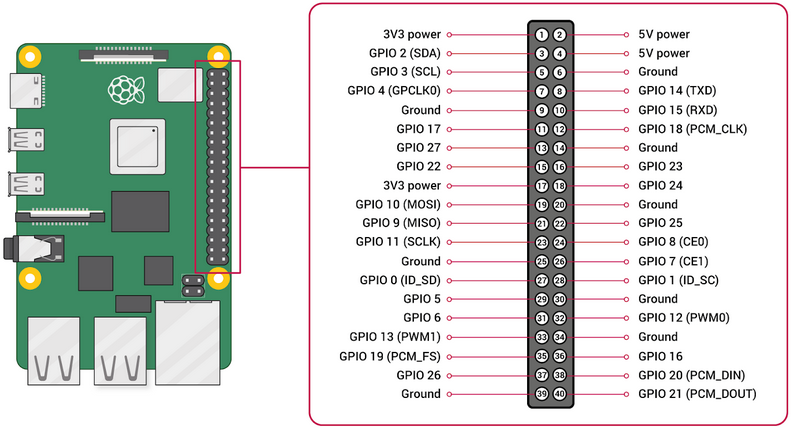
\includegraphics[width=\columnwidth]{raspberry_pi.png}
    \caption{Microprocessor (Raspberry Pi 4B 4GB)}
\end{figure}

Raspberry Pi 4B 4GB RAM model comes packed with, 

\begin{description}
    \item[1.]Quad core Cortex-A72 64-bit @ 1.5 GHz clock and uses ARM v8 architecture, 
    with 4GB LPDDR4-3200 SDRAM.
    \item[2.]2.4 and 5 GHz IEEE 802.11ac wireless wifi hardware.
    \item[3.]2 Micro HDMI ports.
    \item[4.]H.265 (4kp60 decode), H264 (1080p60 decode, 1080p30 encode).
    \item[5.]OpenGL ES 3.0 graphics.
    \item[6.]Micro-SD card slot for loading operating system and data storage.
    \item[7.]4 USB ports.
    \item[8.]Software PWM on all pins and Hardware on GPIO12, GPIO13, GPIO18, GPIO19.
    \item[9.]SPI
    \begin{description}
        \item[-]SPI0 : MOSI (GPIO10), MISO (GPIO9), SCLK (GPIO11), CE0 (GPIO8), CE1 (GPIO7).
        \item[-]SPI1 : MOSI (GPIO20), MISO (GPIO19), SCLK (GPIO21), CE0 (GPIO18), CE1 (GPIO17), CE2 (GPIO16).  
    \end{description}  
\end{description}

\subsection{Mechanical unit}

As discussed in methodology, as the speakers propgates sound in oval shape we need to align the major 
axis of the sound field towards the listener.

Mechanical units assembles with, two servo motors for each speaker (channel)
one for panning and second for tilting.

For this appplication we are using SG90 servos which comes with

\begin{description}
    \item[1.]180\si{\degree} rotation (90 in each direction).
    \item[2.]Torque 2.5 kg-cm
    \item[3.]Volatge 4.8-6 V  
    \item[4.]Speed 0.12 sec/60\si{\degree}
\end{description}

\subsection{Audio processor unit}

Even if we direct the speakers towards listeners direction, it is encessary to adjust the sound
levels of each speaker according to the depth of the listener from each speaker.

Audio processor unit is a hardware with 4 class AB audio amplifiers and 2 two-channel digital 
potentiometers for controlling sound levels of each individual speaker to adjust the sound 
pocket over listener's head (ears).

\*\\Explain the circuit diagram tomorrow*\

\subsection{Speakers}

\*Explain this block little bit more tomorrow\\*\

Final and main component, speaker. Which is mounted on servo and provided with dynamically controlled 
sound using Audio Processor.

\chapter{BLOCK DIAGRAM OF THE SYSTEM}

\end{document}